%%%%%%%%%%%%%%%%%%%%%%%%%%%%%%%%%%%%%%%%%%%%%%%%%%%%%%%%%%%%%%%%%%%%%%%%%%%%%%%%%%%%%%%%%%%%%%
%%%%%%%%%%%%%%%%%%%%%%%%%%%%%%%%%%%%%%%%%%%%%%%%%%%%%%%%%%%%%%%%%%%%%%%%%%%%%%%%%%%%%%%%%%%%%%
%%%%%%%%%%% Estimators
%%%%%%%%%%%%%%%%%%%%%%%%%%%%%%%%%%%%%%%%%%%%%%%%%%%%%%%%%%%%%%%%%%%%%%%%%%%%%%%%%%%%%%%%%%%%%%
%%%%%%%%%%%%%%%%%%%%%%%%%%%%%%%%%%%%%%%%%%%%%%%%%%%%%%%%%%%%%%%%%%%%%%%%%%%%%%%%%%%%%%%%%%%%%%


% \cleardoublepage
\chapter{Estimators}
\label{sec:estimators}
This thesis studies the GPU implementation of data-aided equalizers.
Data-aided equalizers are computed using a channel and noise variance estimates based on a known data sequence in the received signal.
The channel and noise variance estimates are very suseptable to a frequency offset.
The frequency offset must be estimated then removed.
All the estimates are data-aided and thus require finding the known data sequence in the received signal.
A preamble detector is employed to estimate the starting index of each preamble in a set.
Figure \ref{fig:estimatorBlock} shows a block diagram of the estimators in the PAQ project.
The estimators will be briefly explained in Sections \ref{sec:pd} to \ref{sec:noise_variance_estimation}
\begin{figure}
	\caption{A block diagram of the estimation process.}
	\centering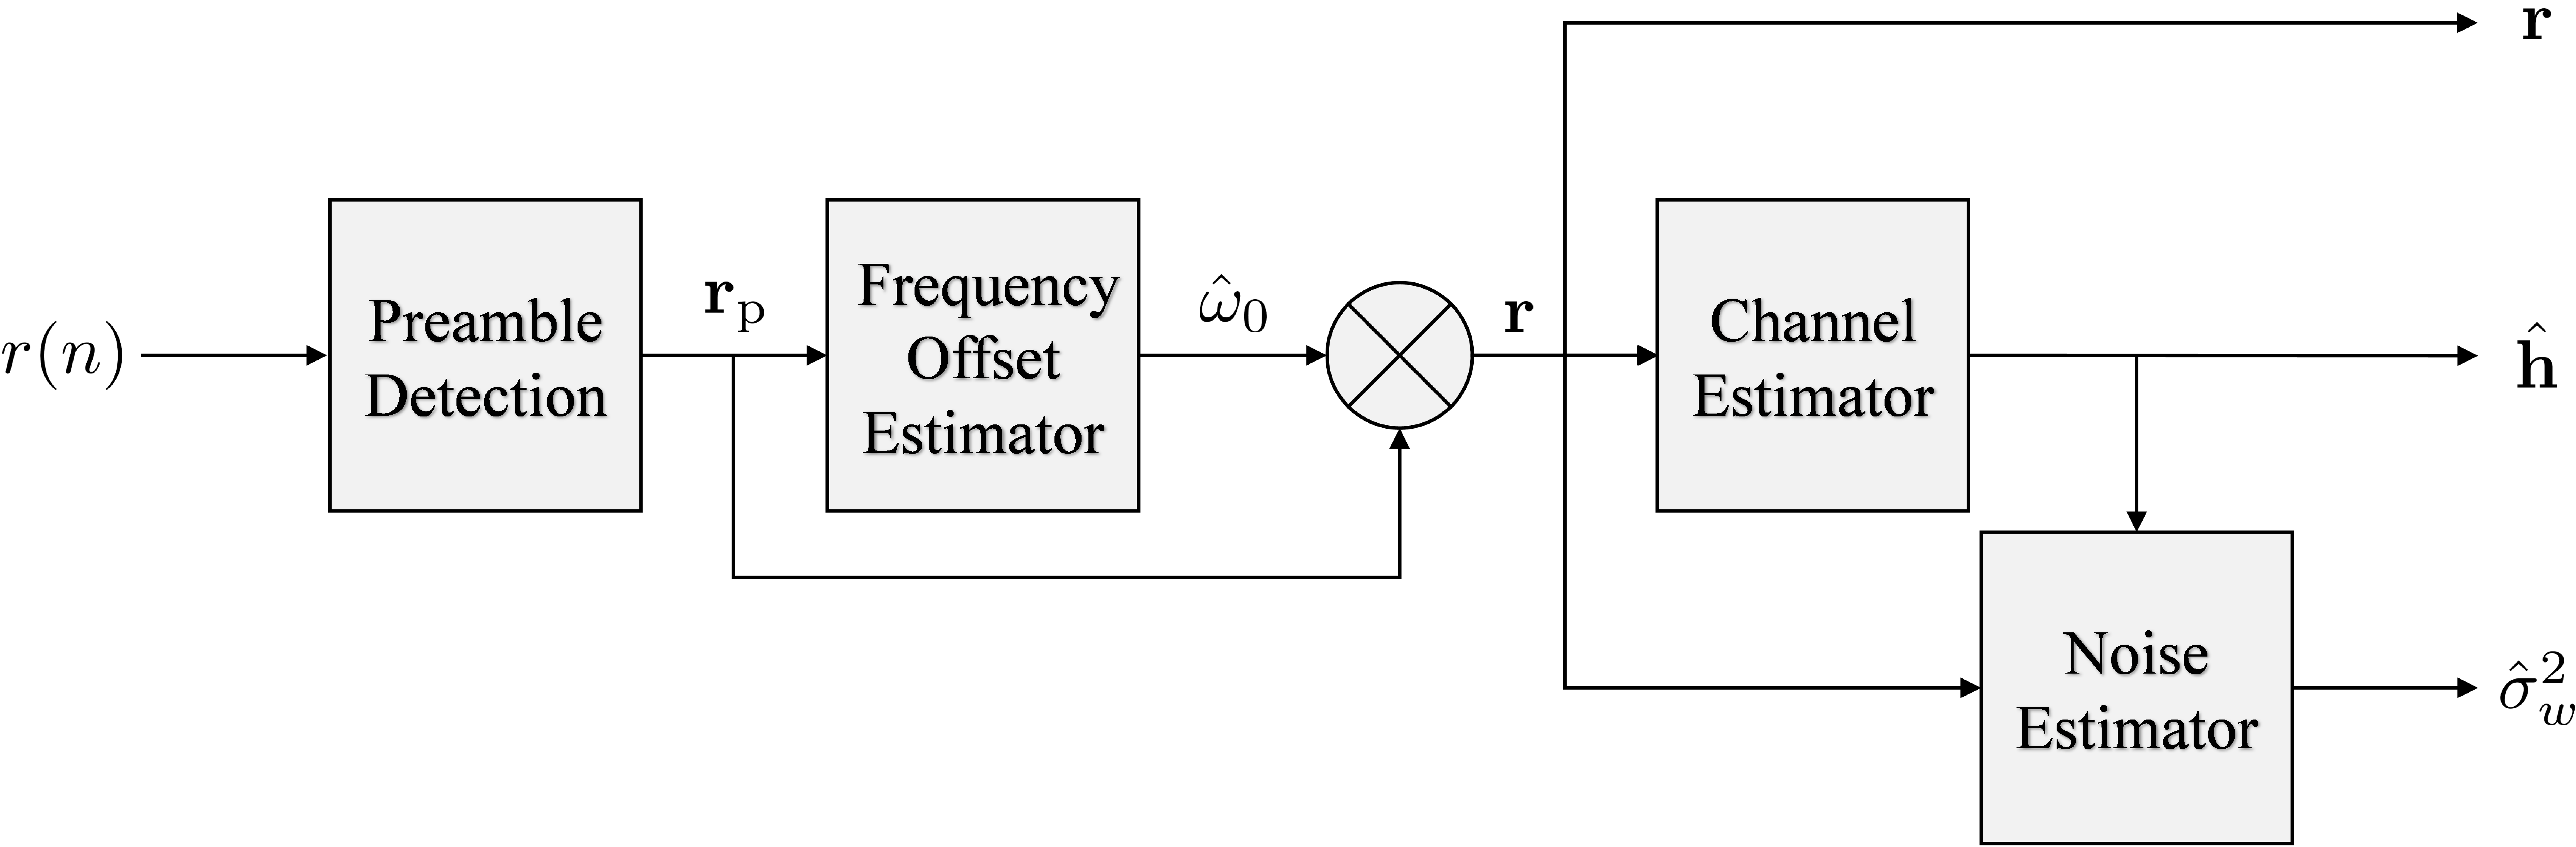
\includegraphics[width=10.33in/100*55]{figures/systemOverview/estimatorBlock.pdf}
	\label{fig:estimatorBlock}
\end{figure}

The data-aided equalizers are then computed and the received samples are equalized.
With the signal equalized, a detection filter is applied and the symbols are detected by a OQPSK symbol by symbol detector.
Figure \ref{fig:ProcessingBlock} shows a block diagram of how the equalizers are computed then applied.
The detection filter and OQPSK detector are explained in Section \ref{sec:oqpsk_detector} but the blocks in the dotted box.
Chapter \ref{chap:eq_eq} will explain the equations for the equalizers and the application of the equalizers and detection filter.
\begin{figure}
	\caption{A block diagram of the equalization and symbol detector process.}
	\centering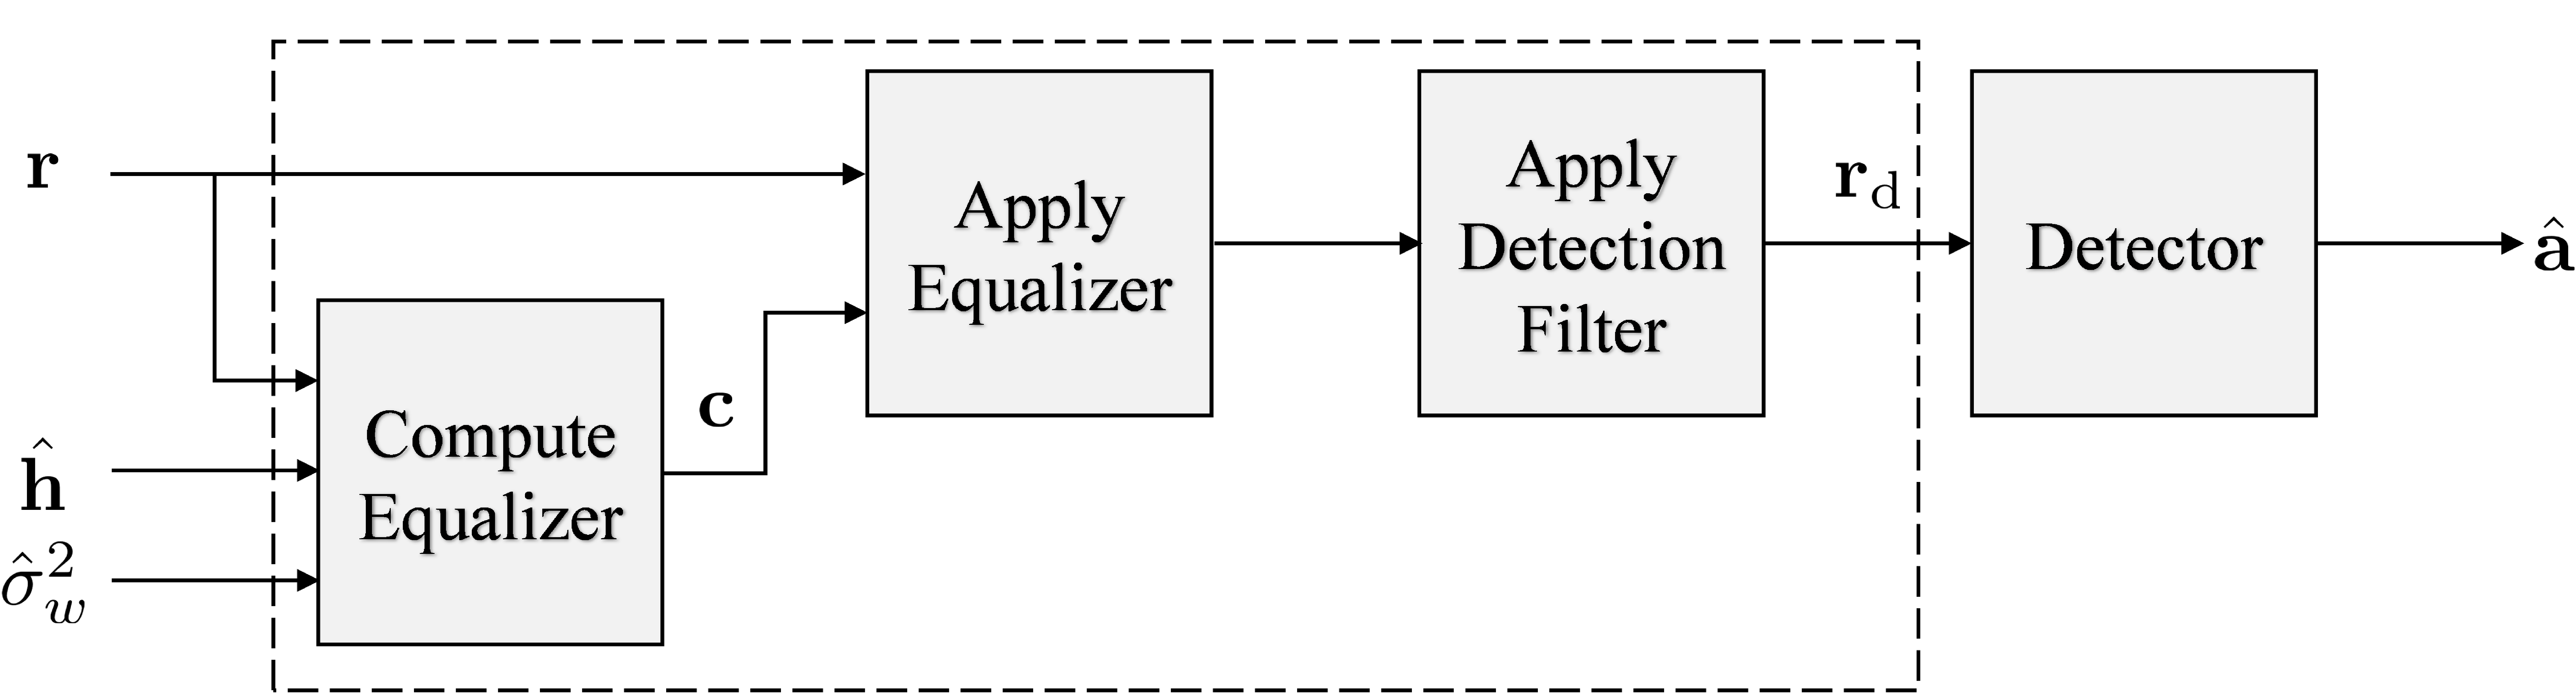
\includegraphics[width=9.35in/100*55]{figures/systemOverview/ProcessingBlock.pdf}
	\label{fig:ProcessingBlock}
\end{figure}

\section{Preamble Detection}
\label{sec:pd}
To compute data-aided preamble assisted equalizers, preambles in the received signal are found then used to estimate various parameters.
The goal of the preamble detection step is to structure the received samples into length $\Lpkt$ packets or batches with the structure shown in Figure \ref{fig:packet}.
Each packet contains $\Lp = 256$ preamble samples, $\Lasm = 136$ ASM samples and $\Ldata = 12288$ data samples.
The full length of a packet is $\Lp + \Lasm + \Ldata = 12672$.

Before the structureing the received samples into packets, the preambles are found using a preamble detector explained in \cite{preamble_detector}.
Equations \eqref{eq:gpu-L-4} through \eqref{eq:gpu-L-pedone-geoghegan-4} have been optimized for GPUs and are implemented directly.
\begin{equation}
	L(u) = \sum_{m=0}^{7}
		\left[ I^2(n,m) + Q^2(n,m) \right]
	\label{eq:gpu-L-4}
\end{equation}
where the inner terms are
\begin{multline}
	I(n,m) \approx \sum_{\ell\in\mathcal{L}_1}r_R(\ell+32m+n)
			- \sum_{\ell\in\mathcal{L}_2}r_R(\ell+32m+n)
			+ \sum_{\ell\in\mathcal{L}_3}r_I(\ell+32m+n)
			- \sum_{\ell\in\mathcal{L}_4}r_I(\ell+32m+n)
			\\
			+ 0.7071 \left[
				\sum_{\ell\in\mathcal{L}_5}r_R(\ell+32m+n)
				- \sum_{\ell\in\mathcal{L}_6}r_R(\ell+32m+n)
			\right. \\
			\left.
				+ \sum_{\ell\in\mathcal{L}_7}r_I(\ell+32m+n)
				- \sum_{\ell\in\mathcal{L}_8}r_I(\ell+32m+n)
			\right],
	\label{eq:gpu-L-pedone-geoghegan-2}
\end{multline}
and
\begin{multline}
	Q(n,m) \approx \sum_{\ell\in\mathcal{L}_1}r_I(\ell+32m+n)
			- \sum_{\ell\in\mathcal{L}_2}r_I(\ell+32m+n)
			\\
			- \sum_{\ell\in\mathcal{L}_3}r_R(\ell+32m+n)
			+ \sum_{\ell\in\mathcal{L}_4}r_R(\ell+32m+n)
			\\
			+ 0.7071 \left[
				\sum_{\ell\in\mathcal{L}_5}r_I(\ell+32m+n)
				- \sum_{\ell\in\mathcal{L}_6}r_I(\ell+32m+n)
			\right. \\
			\left.
				- \sum_{\ell\in\mathcal{L}_7}r_R(\ell+32m+n)
				+ \sum_{\ell\in\mathcal{L}_8}r_R(\ell+32m+n)
			\right]
		\label{eq:gpu-L-pedone-geoghegan-3}
\end{multline}
with
\begin{equation}
	\begin{split}
	\mathcal{L}_1 &= \{ 0, 8, 16, 24 \}\\
	\mathcal{L}_2 &= \{ 4, 20 \}\\
	\mathcal{L}_3 &= \{ 2, 10, 14, 22 \}\\
	\mathcal{L}_4 &= \{ 6, 18, 26, 30 \}\\
	\mathcal{L}_5 &= \{ 1, 7,  9, 15, 17, 23, 25, 31 \}\\
	\mathcal{L}_6 &= \{ 3, 5, 11, 12, 13, 19, 21, 27, 28, 29 \}\\
	\mathcal{L}_7 &= \{ 1, 3,  9, 11, 12, 13, 15, 21, 23 \}\\
	\mathcal{L}_8 &= \{ 5, 7, 17, 19, 25, 27, 28, 29, 31 \}.
\end{split}
\label{eq:gpu-L-pedone-geoghegan-4}
\end{equation}

A correlation peak in $L(u)$ indicate the starting index $k$ of a preamble.
The vector $\mathbf{r}_\text{p}$ in Figure \ref{fig:estimatorBlock} is defined by
\begin{equation}
\mathbf{r}_\text{p} = 
\begin{bmatrix}
r(k) \\ 
\vdots \\ 
r(k+\Lpkt-1)
\end{bmatrix}
=
\begin{bmatrix}
r_\text{p}(0) \\ 
\vdots \\ 
r_\text{p}(\Lpkt-1)
\end{bmatrix}
\end{equation}

\section{Frequency Offset Compensation}
\label{sec:freq_offset_comp}
The frequency offset estimator shown in Figure \ref{fig:estimatorBlock} is the estimator taken from \cite[eq. (24)]{rice2014frequency}.
With the notation adjusted slightly, the frequency offset estimate is
\begin{equation}
	\hat{\omega}_0 = \frac{1}{L_q} \arg\left\{ \sum_{n=i+2L_q}^{i+7L_q-1} r_\text{p}(n)r_\text{p}^\ast(n-L_q)\right\}
	\quad
\text{for} \;
i=1,2,3,4,5.
	\label{eq:jeff-ML-w-final3}
\end{equation}
The frequency offset is estimated for every packet or each vector $\mathbf{r}_\text{p}$.
The frequency offset is compensated for by derotating the packet structured samples by the estimated offset
\begin{equation}
	r(n) = r_\text{p}(n) e^{-j\hat{\omega}_0n}.
	\label{eq:frequency_compensation}
\end{equation}
Equations \eqref{eq:jeff-ML-w-final3} and \eqref{eq:frequency_compensation} are easily implemented into GPUs. 

\section{Channel Estimation}
\label{sec:channel_estimation}
The channel estimator is the ML estimator taken from \cite[eq. 8]{rice-afran-saquib-cole-rhodes-moazzami:2014}.
\begin{equation}
\hat{\mathbf{h}} = \underbrace{ \left( \mathbf{X}^\dag\mathbf{X} \right)^{-1} \mathbf{X}^\dag}_{\mathbf{X}_\text{lpi}}\mathbf{r}
\end{equation}
where $\mathbf{X}$ is a convolution matrix formed from the ideal preamble and ASM samples
and $\mathbf{X}_\text{lpi}$ is the left psudo-inverse of $\mathbf{X}$.
The ML channel estimator is the result of the matrix operation
\begin{equation}
\hat{\mathbf{h}} = \mathbf{X}_\text{lpi} \mathbf{r}.
\end{equation}
The matrix operation $\mathbf{X}_\text{lpi} \mathbf{r}$ is implemented simply and efficiently in GPUs.


\section{Noise Variance Estimation}
\label{sec:noise_variance_estimation}
The noise variance estimator is also taken from \cite[eq. 9]{rice-afran-saquib-cole-rhodes-moazzami:2014}
\begin{equation}
	\hat{\sigma}_w^2 = \frac{1}{2\rho} \left| \mathbf{r}-\mathbf{X}\hat{\mathbf{h}}\right|^2
	\label{eq:ML-s2-final3}
\end{equation}
where
\begin{equation}
	\rho = {\rm Trace} \left\{ \mathbf{I} -  \mathbf{X}\left(\mathbf{X}^\dag\mathbf{X}\right)^{-1}\mathbf{X}^\dag \right\}.
\end{equation}
Equation \eqref{eq:ML-s2-final3} is easily implemented into GPUs.
	

\section{Symbol-by-Symbol Detector}
\label{sec:oqpsk_detector}
The symbol by symbol detector block in Figure \ref{fig:ProcessingBlock} is a Offset Quadrature Phase Shift Keying (OQPSK) detector.
Using the simple OQPSK detector in place of the complex MLSE SOQPSK-TG detector leads to less than $1$dB in bit error rate \cite{perrins:2013}.
\begin{figure}
	\caption{Offset Quadriture Phase Shift Keying symbol by symbol detector.}
	\centering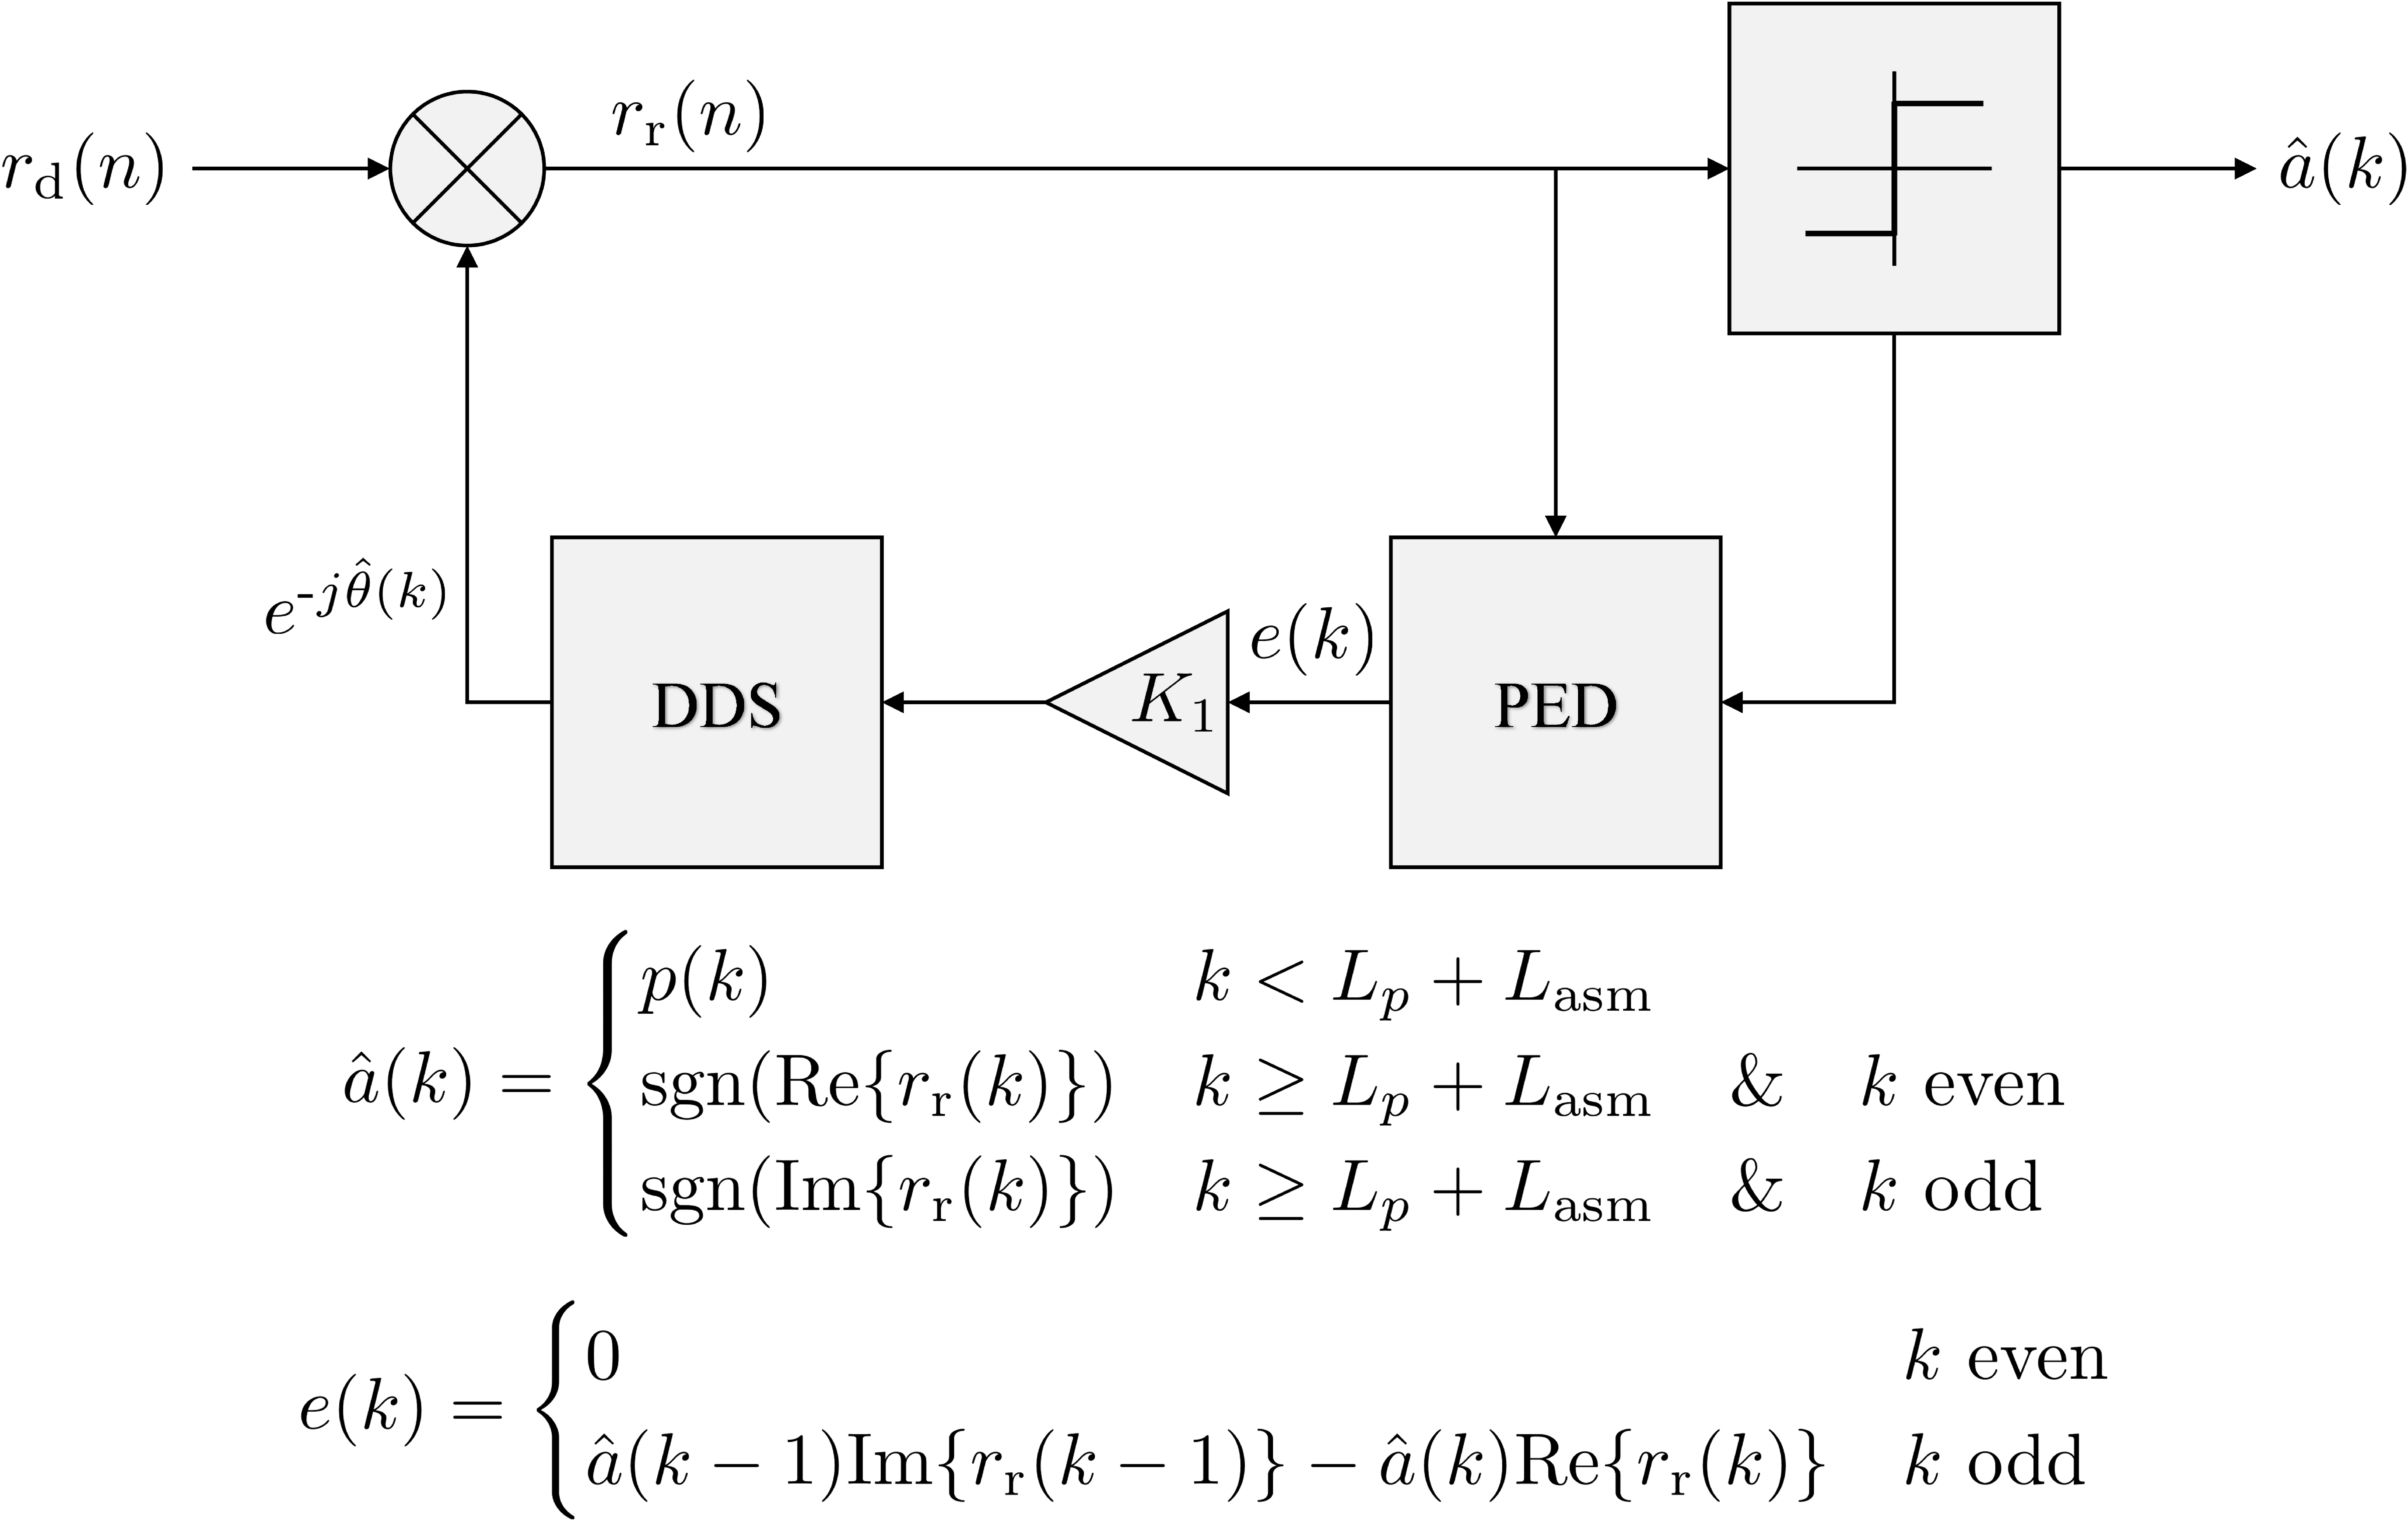
\includegraphics[width=6in]{figures/systemOverview/OQPSK.pdf}
	\label{fig:OQPSK}
\end{figure}

A Phase Lock Loop (PLL) is needed in the OQPSK detector to track out residual frequency offset.
The residual frequency offset results from the frequency offset estimation error.
While phase offset, timing offset and multipath are combated with equalizers, batched based equalizers cannot remove residual frequency offset.
The PLL tracks out the residual frequency offset using a feedback control loop.

Implementing a PLL may not seem feasible in GPUs because the feedback loop cannot be parallelized.
But the PAQ system processes $3104$ batches of data at a time.
The detector and PLL are parallelized on a packet by packet basis.
Running the PLL and detector serially through a full packet of data is relatively fast because each iteration requires only $10$ floating point operations and a few logic decisions.